\chapter{Analysis}
\label{ch:analysis}
In the analysis phase, the product requirements are derived --- defining the client expectations
for the product --- as well as the project constraints --- what the environments
limits about the product. Based on the set of requirements and constraints, a
system overview is produced, capturing the main features and interactions with
the system, as well as its key components.

Then, the system architecture is
devised, comprising both hardware and software domains. Next, the system is
decomposed into subsystems, presenting a deeper analysis over it, comprising its
user mockups, events, use cases diagram, dynamic operation and flow of events.

Lastly, the theoretical foundations are outlined,
providing the basic technical knowledge to undertake the project.
%
% Requirements and constraints
\section{Requirements and Constraints}
\label{sec:req-const}
%
The development requirements are divided into functional and non-functional if they pertain to main functionality or secondary one, respectively. Additionally, the constraints of the project are classified as technical or non-technical.

\subsection{Functional requirements}
\label{sec:funct-requ}
%
\begin{item-c}
\item Advertising through a screen and speakers;
\item Have fragrance diffusion;
\item Take pictures and~\gls{gif}s;
\item Detect a user in range of the device;
\item Contactless user interaction through gesture recognition;
\item Camera feed and facial recognition;
\item Apply brand-specific image filters;
\item Enable sharing multimedia across social media;
\item Provide a remote user interface for brands to purchase and configure the advertisements;
\item Provide a remote user interface for company staff to assess and control
  the MDO local system.
\end{item-c}
%
\subsection{Non-functional requirements}
\label{sec:non-funct-requ}
%
\begin{item-c}
\item Low power consumption;
\item Provide user-friendly interfaces;
\item Have low latency between local system and remote server;
\item Use wireless communication between the local and remote systems.
\end{item-c}
%
\subsection{Technical constraints}
\label{sec:techn-constr}
%
\begin{item-c}
\item Use device drivers;
\item Use Makefiles;
\item Use C/C++;
%\item Develop a~\gls{cps};
\item Use Raspberry Pi as the development board;
\item Use compatible~\gls{hw} with the development board;
\item Use buildroot;
%\item Work with Linux;
\item Social media APIs for sharing multimedia
\item Image filtering through specialized APIs.
\end{item-c}
\subsection{Non-technical constraints}
\label{sec:non-techn-constr}

\begin{item-c}
\item Project duration: one semester (circa 20 weeks); 
\item Pair work flow;
\item Limited budget;
\item Scale model prototype.
\end{item-c}

%The requirements defined the client expectations for the TV remote control,
%namely:
%\begin{item-c}
%\item Remotely operated
%\item Low weight
%\item Powered by batteries
%\item 3 buttons: Power (Off/On); Up and Down for channel selection.
%\item Infrared emitter response time (system output response time): 100 ms
%\item The TV remote may be upgraded in the future to use more buttons
%\end{item-c}
%%
%  %\vspace{-5mm}
%%  
%\section{Constraints}
%\label{sec:constraints}
%The project constraints are the limitations the environment imposes on it, namely:
%\begin{item-c}
%\item the TV remote must contain an infrared emitter (the TV already has an infrared receiver)
%\item The TV remote control must supply the required data frames imposed by the TV
%  manufacturer
%\item Data frames may not be provided by the client
%\item Security concerns are defined by the data frames and the specific
%  communication frequency imposed by the TV manufacturer
%\item 1 week deadline: 14 h
%\item Manpower: 2 people
%\item Budget:
%  \begin{itemize}
%  \item HW (parts acquisition and assembly): fixed costs --- 1 EUR/unit (1000
%    batch production)
%    \begin{itemize}
%    \item TV remote Shell
%    \item TV remote membrane
%    \item Data acquisition \& Infrared emitter PCB
%    \end{itemize}
%  \item Development: project --- 20 EUR per hour per person, totalling 560 EUR +
%    IVA
%  \end{itemize}
%\end{item-c}
%
  %\vspace{-5mm}
%  

%%% Local Variables:
%%% mode: latex
%%% TeX-master: "../../../dissertation"
%%% End:

% System overview
%
\section{System overview}
\label{sec:system-overview}
The system overview presents a global view of the system, considering its main
features, components and interactions. It is not intended to be complete, but
rather provide a basis for the outline of the system architecture.
Fig.~\ref{fig:sys-overview} presents the \gls{mdo} system overview.
%
\begin{figure}[htb!]
\centering
    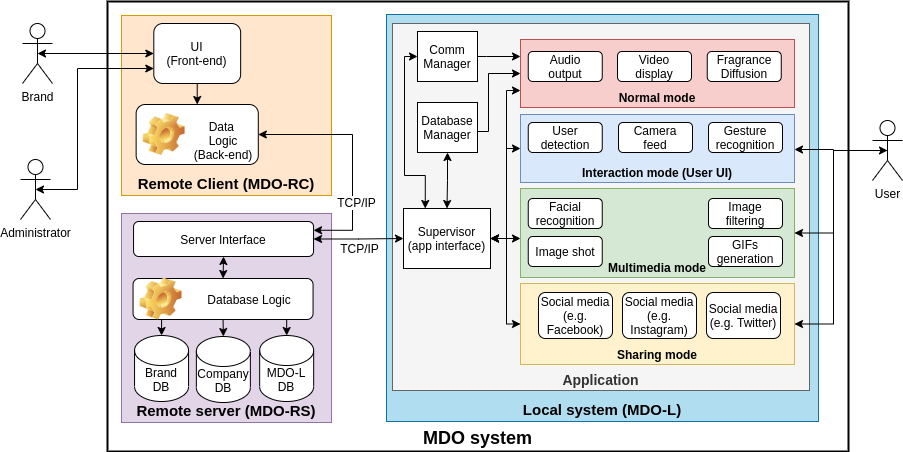
\includegraphics[width=1.0\columnwidth]{./img/sys-overview.png}
  \caption{\gls{mdo} system overview}%
\label{fig:sys-overview}
\end{figure}

Considering the system interactions, three main actors were identified:
\begin{enum-c}
\item \emph{Brand}: represents the brands contracting the advertisement
  services;
\item \emph{Administrator}: the development company staff, which can monitor and
  control the outdoor (administrative privileges).
\item \emph{User}: the user (the target audience of the advertisement)
  interacting with the system.
\end{enum-c}

Considering the data flow across the \textbf{MDO system}, three main subsystems were
identified: \textbf{\gls{mdo-rc}}, \textbf{\gls{mdo-rs}}, and
\textbf{\gls{mdo-l}}. The rational behind this initial decomposition is
explained next.

\subsection{MDO Remote Client}
The \emph{Brand} and \emph{Administrator} members require a remote \gls{ui} (front-end) to
interact with the system: the former to configure the advertisements being
displayed at the \gls{mdo} and purchase them; the latter to remotely monitor and
control the operation of the \gls{mdo}. Thus, it is clear that \emph{an
  authentication mechanism must be provided for the remote \gls{ui}}.

The data is then dispatched to the back-end, where it is processed and feed back
to the \gls{ui} user and/or sent to the remote server, via \gls{tcp-ip}
comprising the data logic component of the \gls{ui}.
%
%
\subsection{MDO Remote Server}
\label{sec:mdo-remote-server}
Although the \gls{mdo-rc} could communicate directly with the \gls{mdo-l}, this
is not desirable or a good architecture mainly due to: communications failure could
result in data loss, compromising the system's integrity; the remote client and
the local system become tightly coupled, meaning the remote client must be aware
of all the available local systems; if the data storage in the local system
fails, the remote client would have to provide the backup information.

Thus, a remote server component is included, providing the access and management
of the system databases, pertaining to the \emph{Brand}, \emph{Company}, and
\emph{MDO Local system}. The first two provide the historical information of the
\texttt{Brand} and \texttt{Administrator} entities, and the last one the information
related to all of the \texttt{\gls{mdo-l}} systems in operation.

The main functions of the \texttt{\gls{mdo-rs}} are:
\begin{item-c}
\item \emph{UI requests responses}: when a \gls{ui} user requests/modifies
  some information from the database, the server must provide/update it.
\item \emph{\gls{mdo-l} monitoring and control}: provide command dispatch and
  feedback to the \texttt{Administrator} staff for remote monitoring and control of
  the device.
\item \emph{\gls{mdo-l} update}: periodically check for start times of each
  \gls{mdo-l} device and transfer the relevant data to it.
\end{item-c}

The server interface is the responsible for managing the requests and respective
responses from the remote client and for periodically send the update data to
all \gls{mdo-l} devices. 
%
%
\subsection{MDO Local system}
\label{sec:mdo-local-system}
The \gls{mdo} local system (MDO-L) is the marketing device, interacting with the user
to display multi-sensory advertisements. As aforementioned in
Section~\ref{sec:prob-stat}, it is comprised of four modes:
\begin{item-c}
\item \emph{normal mode}: the MDO provides sound, video and fragrance
  outputs. It is the default mode.
\item \emph{interaction mode}: When a user approaches the device, the \gls{mdo} will
go into interaction mode, turning on and displaying the camera feed and waiting
for recognizable gestures to provide additional functionalities, such as
brand-specific image filters. This is the \texttt{User} \gls{ui}.
\item \emph{multimedia mode}: in this mode the facial recognition is applied,
  enabling the user to select and apply different brand-specific image filters and take pictures or create a \gls{gif}.
\item \emph{sharing mode}: after a user take a picture or create a \gls{gif}, it
  can share it across social media.
\end{item-c}

The user interaction is considered to be a higher priority activity than the
advertisements, so when a \texttt{User} interacts with the system, the \texttt{normal
mode} is overriden by the \texttt{Interaction mode}, thus, halting the
advertisements.

The \gls{mdo-l} application communicates with the remote server
(\texttt{\gls{mdo-rs}}) through the \texttt{Supervisor} via \gls{tcp-ip}
 to handle requests from \texttt{Administrator} members
to monitor and control the device through the \texttt{Supervisor} or to update
the advertisements. Additionally, the \texttt{Supervisor} oversees the
application mode and the communication (\texttt{Comm Manager}) and database
(\texttt{Database manager}) managers to handle system events.
%
%%% Local Variables:
%%% mode: latex
%%% TeX-master: "../../../dissertation"
%%% End:

% System Architecture
%
\section{System architecture}
\label{sec:system-architecture}
In this section, the system architecture is devised in the \gls{hw} and \gls{sw} components, using the system overview as a starting point. 

\subsection{Hardware architecture}
\label{sec:hardw-arch}
%
The diagram in Fig.\ref{fig:hw-arch} represents an initial hardware big picture in order to facilitate the objective identification.
As it can bee seen, the diagram is divided in four distinguished parts: \emph{External Environment}, \emph{Local System}, \emph{Remote Server} and \emph{Remote Client}.

Firstly, the \texttt{External Environment} represents all the environment that interacts with the system. In this case, these are all its users - normal users, brands and staff.

Secondly, the \texttt{Local System} is composed for the main controller, which is the Raspberry Pi 4B. 
This \gls{mcu} is responsible to controll all the Local System and to establish connection with the remote server through its included WiFi module. 
The board is powered connecting it to the electrical network. 
Then, it has several blocks connected to it:
%
\begin{item-c}
\item \emph{Motion Detection}: Used to detect the users and switch from normal mode to interaction mode;
\item \emph{Fragrance Diffusion Actuator}: used to diffuse the fragrance onto the air;
\item \emph{Camera}: Used to capture image that is then processed;
\item \emph{Speakers}: Used to produce advertisements sounds;
\item \emph{Screen}: Used to produce video clips of advertisements.
\end{item-c}
%

In third place, the \texttt{Remote Server} has a server node running in another machine that can be one computer or a main frame.
The remote server establishes connection with the cloud that has stored all the data from all databases.

Lastly, the \texttt{Remote Client} which can be a computer, a tablet or a smart phone to run the \gls{mdo} management application.
%
\begin{figure}
\centering
    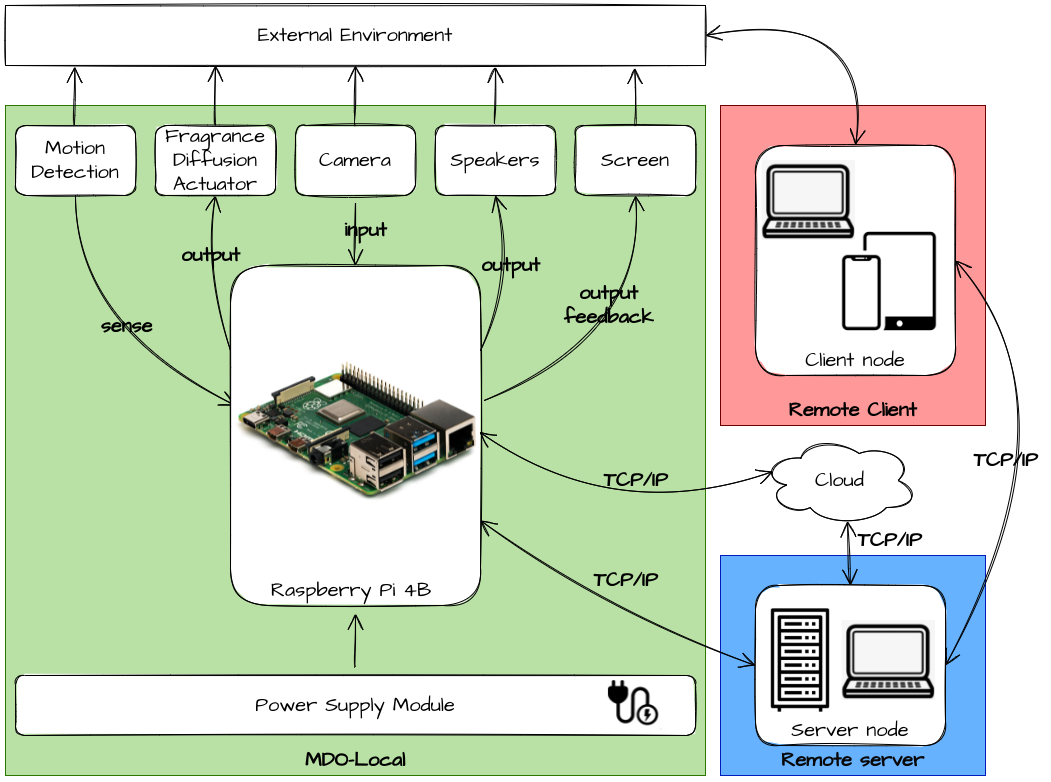
\includegraphics[width=0.9\columnwidth]{./img/HW_Architecture.png}
  \caption{~\gls{hw} Architecture Diagram}%
\label{fig:hw-arch}
\end{figure}
%
%
\subsection{Software architecture}
\label{sec:softw-arch}
In this section the \gls{sw} architecture for \gls{mdo-rc}, \gls{mdo-rs}, and
\gls{mdo-l} subsystems is presented, defining its \gls{sw} stack.

\subsubsection{MDO remote client}
\label{sec:mdo-remote-client}
Fig.~\ref{fig:sw-arch-rc} illustrates the \gls{sw} architecture for the remote
client, representing its \gls{sw} stack.
It is comprised of the following layers:
\begin{item-c}
\item \emph{Application}: contains the remote client application. The
  \texttt{Brand} and \texttt{Admin} members interact with the \gls{ui}, which is
  the visual part of the interface. The \texttt{\gls{ui} engine} is notified and
  handles all \gls{ui} events --- internal or external --- providing the \texttt{UI}
  with feedback for its users. The relevant commands
  are then parsed --- \texttt{Parser} component --- and responded. The commands
  are then translated to the appropriate \gls{db} queries and responded through
  the \texttt{DB Manager}. The \texttt{Comm Manager} is responsible for
  encapsulating the \gls{db} queries into the respective \gls{tcp-ip} frames to
  be sent to the \texttt{Remote Server} as well as unwrap the incoming server
  responses.
\item \emph{Middleware}: contains the \gls{tcp-ip} framework supporting these
  communication protocols as part of \gls{osi} model for internet
  applications. It manages the incoming/outgoing \gls{tcp-ip} frames by
  providing the adequate protocol handshaking and queueing and timing aspects of
  the bytes to send/receive.
\item \emph{OS \& BSP} --- \gls{os} \& \gls{bsp}: it contains the low-level and
  communication drivers required to handle input (keyboard/touch), output
  (screen) and communication to the \texttt{Remote Server}.
\end{item-c}
It should be noted that for desktop and mobile applications, the
\texttt{Middleware} and \texttt{OS \& BSP} layers are usually abstracted by the
\gls{os}, thus, the relevant \gls{api}s should be used.
%
\begin{figure}
\centering
    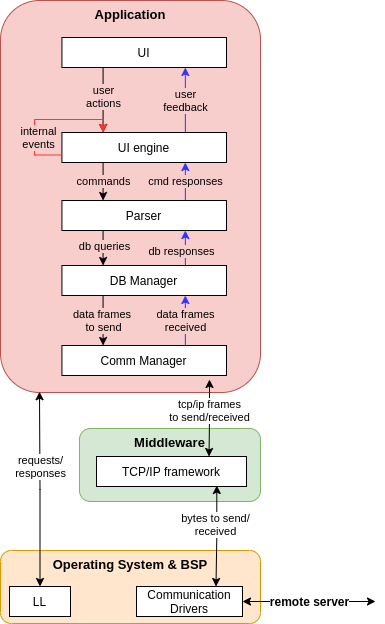
\includegraphics[width=0.55\columnwidth]{./img/sw-arch-rc.png}
  \caption{~\gls{sw} architecture diagram: remote client}%
\label{fig:sw-arch-rc}
\end{figure}

\subsubsection{MDO remote server}
\label{sec:mdo-remote-server-1}
%
Fig.~\ref{fig:sw-arch-rs} illustrates the \gls{sw} stack for architecture for
the remote server.
It is comprised of the following layers:
\begin{item-c}
\item \emph{Application}: contains the remote server application. It provides a
  \gls{cli} to handle \texttt{Remote client} requests.  The \gls{cli} engine
  is notified and handles all \gls{ui} events --- internal or external ---
  providing the appropriate feedback. The relevant commands
  are then parsed --- \texttt{Parser} component --- and responded: \gls{db}
  queries are handled by the \texttt{\gls{rdbms}} issuing \gls{db} transactions;
  other commands received by the \texttt{Remote Client} are handled internally
  and translated, being dispatched to the \texttt{Local
    System} by the \texttt{Comm Manager}  (via \texttt{Communication drivers}). Internal events can also
  trigger the \texttt{\gls{rdbms}} to issue database transactions for the
  \texttt{Remote Client} or \texttt{Local System}.
  The \texttt{Comm Manager} is responsible for wrapping\slash unwrapping the data
  frames received by or sent to the \texttt{Remote Client} or \texttt{Local System}.
\item \emph{Middleware}: contains the \gls{rdbms} framework supporting the
  management of the relational databases using database transactions.
\item \emph{OS \& BSP} --- \gls{os} \& \gls{bsp}: it contains the \texttt{Communication}
  drivers to the handle requests from the \texttt{Remote Client}, and the
  \texttt{File I/O} drivers to manipulate \gls{db} transactions from\slash to storage.
\end{item-c}
%
\begin{figure}
\centering
    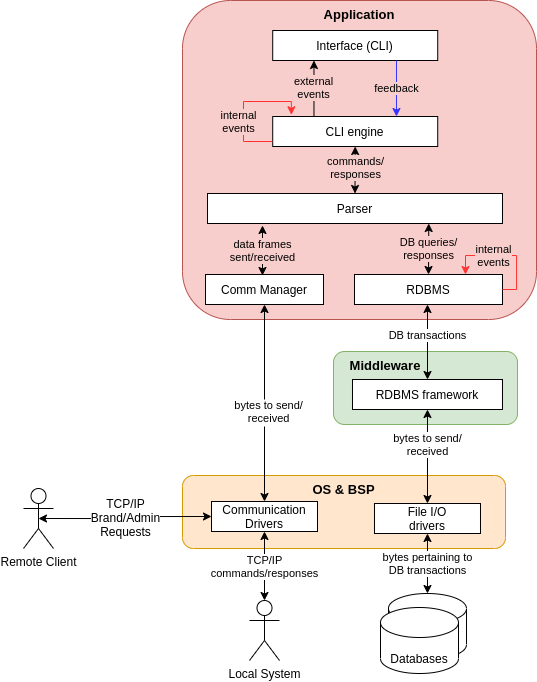
\includegraphics[width=0.55\columnwidth]{./img/sw-arch-rs.png}
  \caption{~\gls{sw} architecture diagram: remote server}%
\label{fig:sw-arch-rs}
\end{figure}
%
\subsubsection{MDO local system}
\label{sec:mdo-local-system-1}




%%% Local Variables:
%%% mode: latex
%%% TeX-master: "../../../dissertation"
%%% End:

% Subsystem decomposition

\section{Subsystem decomposition}
\label{sec:subsyst-decomp}

For each subsystem, do:
1. Events
2. Use cases
3. State machine diagram
4. Sequence diagram

\subsection{Local system}
\label{sec:local-system}

\subsubsection{Events}
\label{sec:events}

\subsubsection{Use cases}
\label{sec:use-cases}

\subsubsection{Dynamic operation}
\label{sec:dyn-oper}
State machine diagram

\subsubsection{Flow of events}
\label{sec:flow-events}
Sequence diagram

\subsection{Remote system}
\label{sec:remote-system}

\subsubsection{Events}
\label{sec:events-1}

\subsubsection{Use cases}
\label{sec:use-cases-1}

\subsubsection{Dynamic operation}
\label{sec:dyn-oper-1}
State machine diagram

\subsubsection{Flow of events}
\label{sec:flow-events-1}
Sequence diagram


%%% Local Variables:
%%% mode: latex
%%% TeX-master: "../../../dissertation"
%%% End:

% Project planning and budget
% \section{Project planning}
\label{sec:project-planning}

\subsection{Budget}
\label{sec:budget}


%%% Local Variables:
%%% mode: latex
%%% TeX-master: "../../../dissertation"
%%% End:

% Theoretical foundations
% \subsection{Waterfall}%
\label{subsec:waterfall}
For the domain-specific design of software the waterfall methodology is used.
The waterfall model (fig.~\ref{fig:waterfall}) represents the first effort to
conveniently tackle the increasing complexity in the software development
process, being credited to Royce, in 1970, the first formal description of the
model, even though he did not coin the term~\cite{sommerville1996software}. It
envisions the optimal method
as a linear sequence of phases, starting from requirement elicitation to system
testing and product shipment~\cite{cusumano1995beyond} with the process flowing
from the top to the bottom, like a cascading waterfall.

In general, the phase sequence is as follows: analysis, design, implementation,
verification and maintenance.
\begin{enumerate}
  \item Firstly, the project requirements are elicited, identifying the key
    requirements and constraints the system being developed must meet from the
    end-user perspective, captured in natural language in a product requirements document.
  \item In the analysis phase, the developer should convert the application
    level knowledge, enlisted as requirements, to the solution domain knowledge
    resulting in analysis models, schema and business rules.
  \item In the design phase, a thorough specification is written allowing the
    transition to the implementation phase, yielding the decomposition in
    subsystems and the software architecture of the system. 
  \item In the implementation stage, the system is developed, following the
    specification, resulting in the source code.
  \item Next, after system assembly and integration, a verification phase occurs
    and system tests are performed, with the systematic discovery and debugging
    of defects.
  \item Lastly, the system becomes a product and, after deployment, the
    maintenance phase start, during the product life time.
\end{enumerate}
While this cycle occurs, several transitions between multiple phases might
happen, since an incomplete specification or new knowledge about the system,
might result in the need to rethink the document.

The advantages of the waterfall model are: it is simple and easy to understand
and use and the phases do not overlap; they are completed sequentially. However,
it presents some drawbacks namely: difficulty to tackle change and high
complexity and the high amounts of risk and uncertainty. However, in the present
work, due to its simplicity, the waterfall model proves its usefulness and will
be used along the project.

As a reference in the sequence of phases and the expected outcomes from each
one, it will be used the chain of development activities and their products
depicted in fig.~\ref{fig:sw-devel-activities} (withdrawn from
\cite{bruegge2004object}).

\begin{figure}[!hbt]
\centering
    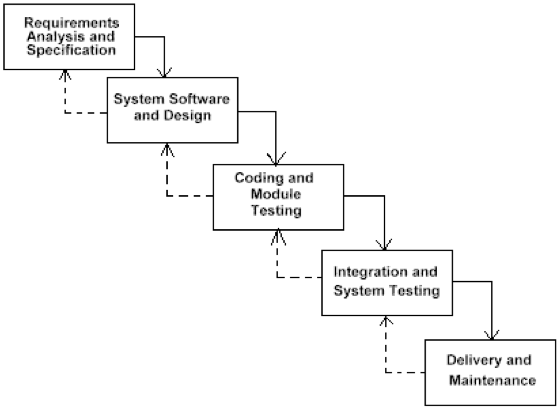
\includegraphics[width=0.6\textwidth]{./img/waterfall.png}
  \caption{Waterfall model diagram}\label{fig:waterfall}
\end{figure}

\subsection{Unified Modeling Language (UML)}
\label{subsec:uml}
To aid the software development process, a notation is required, to articulate
complex ideas succinctly and precisely. The notation chosen was the \gls{uml},
as it provides a spectrum of notations for representing different aspects of a
system and has been accepted as a standard notation in the software
industry~\cite{bruegge2004object}.

The goal of UML is to provide a standard notation that can be used by all
object- oriented methods and to select and integrate the best elements of
precursor software notations, namely \gls{omt}, Booch, and \gls{oose}
~\cite{bruegge2004object}. It provides
constructs for a broad range of systems and activities (e.g., distributed
systems, analysis, system design, deployment). System development focuses on
three different models of the system
(fig.~\ref{fig:sw-devel-activities})~\cite{bruegge2004object}:
\begin{enumerate}
  \item \textbf{\emph{The functional model}}: represented in UML with use case
    diagrams, describes the functionality of the system from the user's point of
    view.
  \item \textbf{\emph{The object model}}: represented in UML with class
    diagrams, describes the structure of the system in terms of objects,
    attributes, associations, and operations.  
  \item \textbf{\emph{The dynamic model}}: represented in UML with interaction
    diagrams, state-machine diagrams, and activity diagrams, describes the
    internal behaviour of the system.
\end{enumerate}

\begin{figure}[!hbt]
\centering
    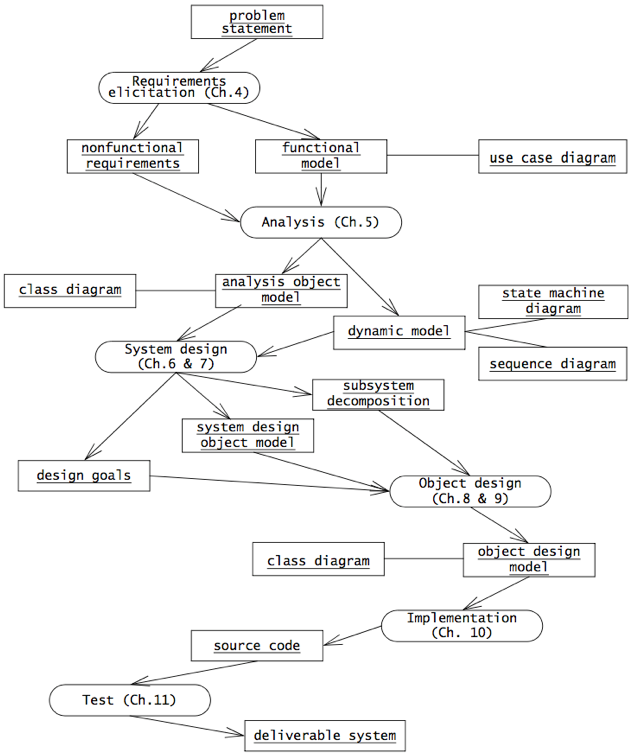
\includegraphics[width=0.7\textwidth]{./img/sw-devel-activities.png}
  \caption{An overview of the object-oriented software engineering development
  and their products. This diagram depicts only logical dependencies among work
  products (withdrawn from~\cite{bruegge2004object})}
\label{fig:sw-devel-activities}
\end{figure}
%%% Local Variables:
%%% mode: latex
%%% TeX-master: "../../../dissertation"
%%% End:

%
%%% Local Variables:
%%% mode: latex
%%% TeX-master: "../../../dissertation"
%%% End:
